\documentclass[
  a4paper,
  oneside,
  BCOR = 10mm,
  DIV = 12,
  12pt,
  headings = normal,
]{scrartcl}

%%% Length calculations
\usepackage{calc}
%%%

%%% Support for color
\usepackage{xcolor}
\definecolor{lightblue}{HTML}{03A9F4}
\definecolor{red}{HTML}{F44336}
%%%

%%% Including graphics
\usepackage{graphicx}
%%%

%%% Font selection
\usepackage{fontspec}

\setromanfont{STIX Two Text}[
  SmallCapsFeatures = {LetterSpace = 8},
]

\setsansfont{IBM Plex Sans}[
  Scale = MatchUppercase,
]

\setmonofont{IBM Plex Mono}[
  Scale = MatchUppercase,
]
%%%

%%% Math typesetting
\usepackage{amsmath}

\usepackage{unicode-math}
\setmathfont{STIX Two Math}

\usepackage{IEEEtrantools}
%%%

%%% List settings
\usepackage{enumitem}
\setlist[enumerate]{
  label*      = {\arabic*.},
  left        = \parindent,
  topsep      = 0\baselineskip,
  parsep      = 0\baselineskip,
  noitemsep, % override itemsep
}
% List settings for levels 2–4
\setlist[enumerate, 2, 3, 4]{
  label*      = {\arabic*.},
  left        = 0em,
  topsep      = 0\baselineskip,
  parsep      = 0\baselineskip,
  noitemsep, % override itemsep
}

\setlist[itemize]{
  label*      = {—},
  left        = \parindent,
  topsep      = 0\baselineskip,
  parsep      = 0\baselineskip,
  itemsep     = 1\baselineskip,
  noitemsep, % override itemsep
}

\setlist[description]{
  font        = {\rmfamily\upshape\bfseries},
  topsep      = 1\baselineskip,
  parsep      = 0\baselineskip,
  itemsep     = 0\baselineskip,
}

%%%

%%% Structural elements typesetting
\setkomafont{pagenumber}{\rmfamily\upshape}
\setkomafont{disposition}{\rmfamily\bfseries}

% Sectioning
\RedeclareSectionCommand[
  beforeskip = -1\baselineskip,
  afterskip  = 1\baselineskip,
  font       = {\normalsize\bfseries\scshape},
]{section}

\RedeclareSectionCommand[
  beforeskip = -1\baselineskip,
  afterskip  = 1\baselineskip,
  font       = {\normalsize\bfseries\itshape},
]{subsection}

\RedeclareSectionCommand[
  beforeskip = -1\baselineskip,
  afterskip  = 1\baselineskip,
  font       = {\normalsize\bfseries},
]{subsubsection}

\RedeclareSectionCommand[
  beforeskip = -1\baselineskip,
  afterskip  = -0.5em,
  font       = {\normalsize\mdseries\scshape\addfontfeatures{Letters = {UppercaseSmallCaps}}},
]{paragraph}
%%%

%%% Typographic enhancements
\usepackage{microtype}
%%%

%%% Language-specific settings
\usepackage{polyglossia}
\setmainlanguage{ukrainian}
\setotherlanguages{english}
%%%

%%% Captions
\usepackage{caption}
\usepackage{subcaption}

% \DeclareCaptionLabelFormat{closing}{#2)}
\captionsetup[subtable]{
  labelformat = simple,
  labelformat = brace,
  justification = RaggedRight,
  singlelinecheck = false,
}

%\captionsetup[subfigure]{labelformat = closing}

\captionsetup[table]{
  aboveskip = 0\baselineskip,
  belowskip = 0\baselineskip,
}

\captionsetup[figure]{
  aboveskip = 1\baselineskip,
  belowskip = 0\baselineskip,
}

\captionsetup[subfigure]{
  labelformat = simple,
  labelformat = brace,
  justification = RaggedRight,
  singlelinecheck = false,
}
%%%

%%% Hyphenated ragged typesetting
\usepackage{ragged2e}
%%%

%%% Table typesetting
\usepackage{booktabs}
\usepackage{longtable}

\usepackage{multirow}

\usepackage{array}
\newcolumntype{v}[1]{>{\RaggedRight\arraybackslash\hspace{0pt}}p{#1}}
\newcolumntype{b}[1]{>{\Centering\arraybackslash\hspace{0pt}}p{#1}}
\newcolumntype{n}[1]{>{\RaggedLeft\arraybackslash\hspace{0pt}}p{#1}}
%%%

%%% Drawing
\usepackage{tikz}
\usepackage{tikzscale}
\usetikzlibrary{arrows.meta} % Stealth arrow tips
\usetikzlibrary{backgrounds} % Stealth arrow tips
\usetikzlibrary{datavisualization.formats.functions}
\usetikzlibrary{datavisualization}
\usetikzlibrary{fit}
\usetikzlibrary{graphdrawing}
\usegdlibrary{trees}
\usetikzlibrary{graphs}
\usetikzlibrary{intersections}
\usetikzlibrary{patterns}
\usetikzlibrary{positioning}
\usetikzlibrary{shapes.geometric}
\usetikzlibrary{quotes}

\usepackage{pgfplots}
\usepgfplotslibrary{fillbetween}
%%%

%%% SI units typesetting
\usepackage{siunitx}
\sisetup{
  output-decimal-marker = {,},
  exponent-product      = {\cdot},
  inter-unit-product    = \ensuremath{{} \cdot {}},
  per-mode              = symbol,
}
%%%

% Code Highlighting
\usepackage{minted}
\setmintedinline{
  style = bw,
  breaklines,
}

\newminted[bashterm]{text}{%
  autogobble,%
  breaklines,%
  style=bw,%
}

\newminted[codegeneric]{text}{%
  autogobble,%
  style=bw,%
  breaklines,%
  fontsize=\small,%
}

\newmintinline{bash}{%
}

\newmintinline[minttext]{text}{%
  breaklines,%
  breakanywhere,%
}

%%% Framing code listings
\usepackage{tcolorbox}
\tcbuselibrary{breakable}
\tcbuselibrary{minted}
\tcbuselibrary{skins}

% Text file listing
\newtcblisting[
  auto counter,
  list inside,
  number within = section,
]{listingplaintext}[3][]{%
  minted language = text,
  minted style    = bw,
  minted options  = {
    autogobble,
    linenos,
    tabsize = 4,
    breaklines,
    breakanywhere,
    fontsize = \footnotesize,
  },
  empty,
  sharp corners,
  coltitle = black,
  borderline horizontal = {1pt}{0pt}{black},
  titlerule = {0.5pt},
  titlerule style = {
    black,
  },
  toptitle = 0.3em,
  bottomtitle = 0.3em,
  before skip      = \intextsep,
  after  skip      = \intextsep,
  title            = {Лістинг \thetcbcounter: #2},
  list entry       = {\protect\numberline{\thetcbcounter}#2},
  left = 0em,
  right = 0em,
  %
  listing only,
  breakable,
  %
  label = {#3},%
}

\newtcbinputlisting[
  use counter from = listingplaintext,
  list inside,
  number within = section
]{\inputplaintext}[4][]{%
  minted language = text,
  minted style    = bw,
  minted options  = {
    autogobble,
    linenos,
    tabsize = 4,
    breaklines,
    breakanywhere,
    fontsize = \footnotesize,
  },
  empty,
  sharp corners,
  coltitle = black,
  borderline horizontal = {1pt}{0pt}{black},
  titlerule = {0.5pt},
  titlerule style = {
    black,
  },
  toptitle = 0.3em,
  bottomtitle = 0.3em,
  before skip      = \intextsep,
  after  skip      = \intextsep,
  title            = {Лістинг \thetcbcounter: #3},
  list entry       = {\protect\numberline{\thetcbcounter}#3},
  left = 0em,
  right = 0em,
  %
  listing file={#2},
  listing only,
  breakable,
  %
  label = {#4}
}

\newtcblisting[
  use counter from = listingplaintext,
  list inside,
  number within = section,
]{listingpython}[3][]{%
  minted language = python,
  minted style    = bw,
  minted options  = {
    autogobble,
    linenos,
    tabsize = 4,
    breaklines,
    breakanywhere,
    fontsize = \footnotesize,
  },
  empty,
  sharp corners,
  coltitle = black,
  borderline horizontal = {1pt}{0pt}{black},
  titlerule = {0.5pt},
  titlerule style = {
    black,
  },
  toptitle = 0.3em,
  bottomtitle = 0.3em,
  before skip      = \intextsep,
  after  skip      = \intextsep,
  title            = {Лістинг \thetcbcounter: #2},
  list entry       = {\protect\numberline{\thetcbcounter}#2},
  left = 0em,
  right = 0em,
  %
  listing only,
  breakable,
  %
  label = {#3},
  %
  #1%
}

\newtcbinputlisting[
  use counter from = listingplaintext,
  list inside,
  number within = section
]{\inputpython}[4][]{%
  minted language = python,
  minted style    = bw,
  minted options  = {
    autogobble,
    linenos,
    tabsize = 4,
    breaklines,
    breakanywhere,
    fontsize = \footnotesize,
  },
  empty,
  sharp corners,
  coltitle = black,
  borderline horizontal = {1pt}{0pt}{black},
  titlerule = {0.5pt},
  titlerule style = {
    black,
  },
  toptitle = 0.3em,
  bottomtitle = 0.3em,
  before skip      = \intextsep,
  after  skip      = \intextsep,
  title            = {Лістинг \thetcbcounter: #3},
  list entry       = {\protect\numberline{\thetcbcounter}#3},
  left = 0em,
  right = 0em,
  %
  listing file={#2},
  listing only,
  breakable,
  %
  label = {#4}
}

\newtcbinputlisting[
  use counter from = listingplaintext,
  list inside,
  number within = section
]{\inputada}[4][]{%
  minted language = ada,
  minted style    = bw,
  minted options  = {
    autogobble,
    linenos,
    tabsize = 4,
    breaklines,
    breakanywhere,
    fontsize = \footnotesize,
  },
  empty,
  sharp corners,
  coltitle = black,
  borderline horizontal = {1pt}{0pt}{black},
  titlerule = {0.5pt},
  titlerule style = {
    black,
  },
  toptitle = 0.3em,
  bottomtitle = 0.3em,
  before skip      = \intextsep,
  after  skip      = \intextsep,
  title            = {Лістинг \thetcbcounter: #3},
  list entry       = {\protect\numberline{\thetcbcounter}#3},
  left = 0em,
  right = 0em,
  %
  listing file={#2},
  listing only,
  breakable,
  %
  label = {#4}
}

% Linux command-line listing
\newtcblisting{linuxterm}%
{%
  % Syntax highlighing options
  listing only,%
  minted language = bash,%
  minted options={%
    autogobble,%
    linenos%
  },%
  % Presentation options
  empty,%
  %% Margins
  sharp corners,%
  toptitle = 0.0em,%
  bottomtitle = 0.0em,%
  left = 0em,%
  right = 0em,%
  before skip = \intextsep,%
  after skip = \intextsep,%
}

\newtcblisting{linuxtermout}%
{%
  % Syntax highlighing options
  listing only,%
  minted language = text,%
  minted options={%
    autogobble,%
    linenos%
  },%
  % Presentation options
  empty,%
  %% Margins
  sharp corners,%
  toptitle = 0.0em,%
  bottomtitle = 0.0em,%
  left = 0em,%
  right = 0em,%
  before skip = \intextsep,%
  after skip = \intextsep,%
}

% Dockerfile listings
\newtcblisting[
  use counter from = listingplaintext,
  list inside,
  number within = section,
]{listingdocker}[3][]{%
  minted language = dockerfile,
  minted style    = bw,
  minted options  = {
    autogobble,%
    linenos,
    tabsize = 4,
    breaklines,
    breakanywhere,
    fontsize = \footnotesize,
  },
  empty,
  sharp corners,
  coltitle = black,
  borderline horizontal = {1pt}{0pt}{black},
  titlerule = {0.5pt},
  titlerule style = {
    black,
  },
  toptitle = 0.3em,
  bottomtitle = 0.3em,
  before skip      = \intextsep,
  after  skip      = \intextsep,
  title            = {Лістинг \thetcbcounter: #2},
  list entry       = {\protect\numberline{\thetcbcounter}#2},
  left = 0em,
  right = 0em,
  %
  listing only,
  breakable,
  %
  label = {#3},%
}

% Docker Compose listings
\newtcblisting[
  use counter from = listingplaintext,
  list inside,
  number within = section,
]{listingdockercompose}[3][]{%
  minted language = yaml,
  minted style    = bw,
  minted options  = {
    autogobble,%
    linenos,
    tabsize = 4,
    breaklines,
    breakanywhere,
    fontsize = \footnotesize,
  },
  empty,
  sharp corners,
  coltitle = black,
  borderline horizontal = {1pt}{0pt}{black},
  titlerule = {0.5pt},
  titlerule style = {
    black,
  },
  toptitle = 0.3em,
  bottomtitle = 0.3em,
  before skip      = \intextsep,
  after  skip      = \intextsep,
  title            = {Лістинг \thetcbcounter: #2},
  list entry       = {\protect\numberline{\thetcbcounter}#2},
  left = 0em,
  right = 0em,
  %
  listing only,
  breakable,
  %
  label = {#3},%
}


% Customize minted line numbers
\renewcommand{\theFancyVerbLine}{\ttfamily\scriptsize\arabic{FancyVerbLine}}

%%%

%%% Typeset menus and keys
\usepackage{menukeys}[
  os=win,
]
%%%

%%% Links and hyperreferences
\usepackage{hyperref}
\hypersetup{
  bookmarksnumbered = true,
  colorlinks      = false,
  linkbordercolor = red,
  urlbordercolor  = lightblue,
  pdfborderstyle  = {/S/U/W 1.5},
}
%%%

%%% Length adjustment

% Set baselineskip, default is 14.5 pt
\linespread{1.068966} % ~15.5 pt
\setlength{\emergencystretch}{1em}
\setlength{\parindent}{1.5em}
\newlength{\gridunitwidth}
\setlength{\gridunitwidth}{\textwidth / 12}
%%%

%%% Custom commands
\newcommand{\allcaps}[1]{%
  {%
    \addfontfeatures{%
      Letters = UppercaseSmallCaps,
      LetterSpace = 8,%
    }%
    #1%
  }%
}
\newcommand{\filename}[1]{\texttt{#1}}
\newcommand{\progname}[1]{\texttt{#1}}
\newcommand{\commandname}[1]{\texttt{#1}}
\newcommand{\modulename}[1]{\texttt{#1}}
\newcommand{\transeng}[1]{{англ.}~\textit{\textenglish{#1}}}
%%%

%%% Custom math commands
\newcommand{\longvar}[1]{\mathit{#1}}
\newcommand{\vect}[1]{\mathbfit{#1}}
\newcommand{\matr}[1]{\mathbfit{#1}}

\newcommand{\logequiv}{\mathrel{\Longleftrightarrow}} % Logically equivalent

\DeclareMathOperator*{\minimize}{min} % minimize for linear programs
%%%

%%% Custom drawing commands
\makeatletter
\newcommand{\Distance}[3]{% % from https://tex.stackexchange.com/q/56353/121799
\tikz@scan@one@point\pgfutil@firstofone($#1-#2$)\relax  
\pgfmathsetmacro{#3}{veclen(\the\pgf@x,\the\pgf@y)}
}% Explanation: the calc library allows us, among other things, to add and
% subtract points, so ($#1-#2$) is simply the difference between the points
% #1 and #2. The combination \tikz@scan@one@point\pgfutil@firstofone extracts
% the coordinates of the new point and stores them in \pgf@x and \pgf@y.
% They get fed in veclen, and \pgfmathsetmacro stores the result in #3.
% EDIT: included fudge factor, see https://tex.stackexchange.com/a/22702/121799
\makeatother
%%%

\begin{document}

\begin{titlepage}
    \begin{center}
      Міністерство освіти і~науки України\\
      Національний авіаційний університет\\
      Факультет кібербезпеки, комп'ютерної та~програмної інженерії\\
      Кафедра комп'ютеризованих систем управління

      \vspace{\fill}
        Лабораторна робота №~1.5\\
        з~дисципліни «Паралельні і~розподілені обчислення»\\
				на~тему «Обмін повідомленнями. Бібліотека \textenglish{\allcaps{MPI}}»

      \vspace{\fill}

      \begin{flushright}
        Виконав:\\
        студент \allcaps{ФККПІ}\\
        групи \allcaps{СП}-425\\
        Клокун В.\,Д.\\
        Перевірив:\\
        Корочкін О.\,В.
      \end{flushright}

      Київ 2019
    \end{center}
  \end{titlepage}

  \section{Завдання роботи}
    Розробити програму для~заданої паралельної комп'ютерної системи із~локальною пам'яттю~(рис.~\ref{fig:task-sys}).

    \begin{figure}[!htbp]
      \centering
      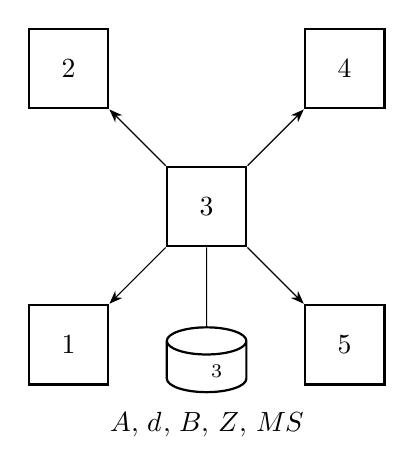
\begin{tikzpicture}[
        iod/.style = {
          draw,
					thick,
          cylinder,
          shape border rotate = 90,
          minimum width = \gridunitwidth,
          aspect = 0.5,
        },
        thread/.style = {
          draw,
					thick,
          rectangle,
          minimum width = \gridunitwidth,
          minimum height = \gridunitwidth,
        },
				>=Stealth,
      ]
				% Leader node
        \node (t3) [
          thread,
          anchor = north west,
        ] {3};

        \node (iod3) [
          iod,
          below = of t3.south,
          anchor = top,
        ] {$\text{ПВВ}_{3}$};

        \node (vars3) [
          below = 0.25 \baselineskip of iod3,
        ] {$A, \, d, \, B, \, Z, \, MS$};

				% Followers
        \node (t1) [
          thread,
          below left = 1\gridunitwidth of t3.south west,
          anchor = north east,
        ] {1};

        \node (t2) [
          thread,
          above left = 1\gridunitwidth of t3.north west,
          anchor = south east,
        ] {2};

        \node (t4) [
          thread,
          above right = 1\gridunitwidth of t3.north east,
          anchor = south west,
        ] {4};

        \node (t5) [
          thread,
          below right = 1\gridunitwidth of t3.south east,
          anchor = north west,
        ] {5};

        % \draw [->] (mem) -- (t1) -- (iod1);
        % \draw [->] (mem) -- (t1);
        % \draw [->] (mem) -- (t2) -- (iod2);
        % \draw [->] (mem) -- (t3) -- (iod3);
        % \draw [->] (mem) -- (t4) -- (iod4);
				\draw [->] (t3) -- (t1) ;
				\draw [->] (t3) -- (t2) ;
				\draw [->] (t3) -- (t4) ;
				\draw [->] (t3) -- (t5) ;
				\draw  (t3) -- (iod3) ;
      \end{tikzpicture}
      \caption{Задана паралельна комп'ютерна система зі~спільною пам'яттю}
      \label{fig:task-sys}
    \end{figure}

    Програма, розроблена для~даної системи, повинна обчислювати значення виразу: $A = d \cdot B + Z \cdot MS$.

  \section{Хід~роботи}
    \subsection{Побудова паралельного алгоритму}
      Щоб~паралельно обчислити значення виразу $A = d \cdot B + Z \cdot MS$, складаємо паралельний алгоритм:
      \begin{enumerate}
				\item $A_{H} = d \cdot B_{H} + Z \cdot MS_{H}$.
      \end{enumerate}
			Паралельний алгоритм реалізуємо на~мові програмування~\textenglish{Python} з~використанням програмного інтерфейсу~\textenglish{\allcaps{MPI}}, реалізованого бібліотекою~\textenglish{Microsoft~\allcaps{MPI}}. Щоб~отримати доступ до~бібліотеки~\textenglish{Microsoft~\allcaps{MPI}} з~програми, написаною мовою~\textenglish{Python}, використаємо обгортку~\textenglish{mpi4py}.

    \subsection{Розробка алгоритмів потоків}
			Розробивши паралельний алгоритм, переходимо до~розробки алгоритмів задач. Представимо алгоритми у~вигляді таблиці~(табл.~\ref{tab:parallel-algos}).

			\begin{table}[!htbp]
				\caption{Паралельні алгоритми задач}
				\label{tab:parallel-algos}
				\begin{subtable}[b]{6 \gridunitwidth - 1em / 2}
					\caption{$T1$}
					\begin{tabular}{
						v{\columnwidth - 2\tabcolsep}
					}
						\toprule
							Дія\\
						\midrule
							Отримати $d$, $B$, $Z$, $MS$ від~$T3$\\
							Обчислити $A_{H} = d \cdot B_{H} + Z \cdot MS_{H}$\\
							Відправити $A_{H}$ в~$T3$\\
						\bottomrule
					\end{tabular}
				\end{subtable}%
				\hspace{1em}
				\begin{subtable}[b]{6 \gridunitwidth - 1em / 2}
					\caption{$T2$}
					\begin{tabular}{
						v{\columnwidth - 2\tabcolsep}
					}
						\toprule
							Дія\\
						\midrule
							Отримати $d$, $B$, $Z$, $MS$ від~$T3$\\
							Обчислити $A_{H} = d \cdot B_{H} + Z \cdot MS_{H}$\\
							Відправити $A_{H}$\\
						\bottomrule
					\end{tabular}
				\end{subtable}
				\begin{subtable}[b]{6 \gridunitwidth - 1em / 2}
					\caption{$T4$}
					\begin{tabular}{
						v{\columnwidth - 2\tabcolsep}
					}
						\toprule
							Дія\\
						\midrule
						Отримати $d$, $B$, $Z$, $MS$ від~$T3$\\
						Обчислити $A_{H} = d \cdot B_{H} + Z \cdot MS_{H}$\\
						Відправити $A_{H}$\\
						\bottomrule
					\end{tabular}
				\end{subtable}%
				\hspace{1em}
				\begin{subtable}[b]{6 \gridunitwidth - 1em / 2}
					\caption{$T5$}
					\begin{tabular}{
						v{\columnwidth - 2\tabcolsep}
					}
						\toprule
							Дія\\
						\midrule
							Отримати $d$, $B$, $Z$, $MS$ від~$T3$\\
							Обчислити $A_{H} = d \cdot B_{H} + Z \cdot MS_{H}$\\
							Відправити $A_{H}$\\
						\bottomrule
					\end{tabular}
				\end{subtable}
				\begin{subtable}[b]{6 \gridunitwidth - 1em / 2}
					\caption{$T3$}
					\begin{tabular}{
						v{\columnwidth - 2\tabcolsep}
					}
						\toprule
							Дія\\
						\midrule
							Ввести $d$, $B$, $Z$, $MS$\\
							Відправити $d$, $B$, $Z$, $MS$ в~$T1$, $T2$, $T4$, $T5$\\
							Отримати $A_{H}$ від~$T1$, $T2$, $T4$, $T5$\\
							Обчислити $A_{H} = d \cdot B_{H} + Z \cdot MS_{H}$\\
							Вивести $A$\\
						\bottomrule
					\end{tabular}
				\end{subtable}
			\end{table}

    \subsection{Розробка структурної схеми взаємодії задач}
      Після розробки алгоритмів потоків, розроблюємо структурну схему взаємодії задач~(рис.~\ref{fig:struct-interaction}).

      \begin{figure}[!htbp]
        \centering
        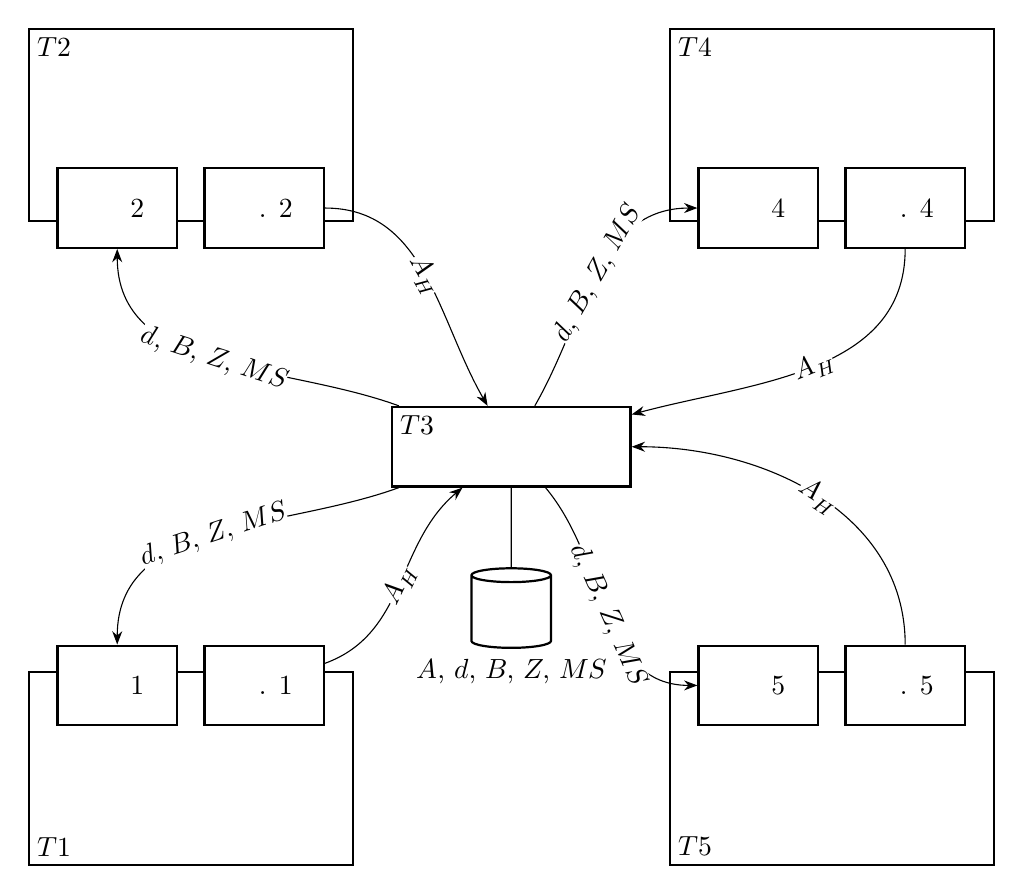
\begin{tikzpicture}[
						resource/.style = {
							draw,
							thick,
						},
						thread/.style = {
							rectangle,
							thick,
							minimum width = 3 \gridunitwidth,
							minimum height = 1 \gridunitwidth,
						},
						syncobj/.style = {
							draw,
							rectangle,
							fill = white,
							thick,
							minimum width = 1.5 \gridunitwidth,
							minimum height = 1 \gridunitwidth,
						},
						iod/.style = {
							draw,
							thick,
							cylinder,
							shape border rotate = 90,
							minimum width = \gridunitwidth,
							minimum height = \gridunitwidth,
							aspect = 0.75,
						},
						edgelabel/.style = {
							fill = white,
							inner sep = 0em,
							pos = 0.5,
						},
						every edge/.append style = {
							sloped,
						},
						threadfit/.style = {
							draw,
							thick,
							inner xsep = 1em,
							inner ysep = 2em,
						},
						>=Stealth,
        ]
					% Leader node
					\node [
						thread,
						draw,
						label = {
							[anchor = north west]north west:$T3$
						}
					] (T3) at (0, 0) {};
					\node [
						iod,
						below = 1 \gridunitwidth of T3.south,
						anchor = top,
						label = {
							below:$A$, $d$, $B$, $Z$, $MS$
						}
					] (TD3) {};

					% Follower nodes
					\node [
						thread,
						below left = 3 \gridunitwidth and 1 \gridunitwidth of T3.south west,
						anchor = north east,
					] (T1) {};
					\node [
						syncobj,
						above left = 0em and 0.5em of T1.north west,
						anchor = south west,
					] (TD1) {Дані 1};
					\node [
						syncobj,
						above right = 0em and 0.5em of T1.north east,
						anchor = south east,
					] (TR1) {Рез. 1};

					\node [
						thread,
						above left = 3 \gridunitwidth and 1 \gridunitwidth of T3.north west,
						anchor = south east,
					] (T2) {};
					\node [
						syncobj,
						below left = 0em and 0.5em of T2.south west,
						anchor = north west,
					] (TD2) {Дані 2};
					\node [
						syncobj,
						below right = 0em and 0.5em of T2.south east,
						anchor = north east,
					] (TR2) {Рез. 2};

					\node [
						thread,
						above right = 3 \gridunitwidth and 1 \gridunitwidth of T3.north east,
						anchor = south west,
					] (T4) {};
					\node [
						syncobj,
						below left = 0em and 0.5em of T4.south west,
						anchor = north west,
					] (TD4) {Дані 4};
					\node [
						syncobj,
						below right = 0em and 0.5em of T4.south east,
						anchor = north east,
					] (TR4) {Рез. 4};

					\node [
						thread,
						below right = 3 \gridunitwidth and 1 \gridunitwidth of T3.south east,
						anchor = north west,
					] (T5) {};
					\node [
						syncobj,
						above left = 0em and 0.5em of T5.north west,
						anchor = south west,
					] (TD5) {Дані 5};
					\node [
						syncobj,
						above right = 0em and 0.5em of T5.north east,
						anchor = south east,
					] (TR5) {Рез. 5};

					\begin{scope}[on background layer]
						% T1 fit
						\node [
							threadfit,
							fit= {(TD1) (TR1)},
							yshift = -3em,
							label = {
								[anchor = south west]south west:$T1$
								}
						] (T1fit) {};

						% T5 fit
						\node [
							threadfit,
							fit= {(TD5) (TR5)},
							yshift = -3em,
							label = {
								[anchor = south west]south west:$T5$
								}
							] (T5fit) {};

						% T2 fit
						\node [
							threadfit,
							fit= {(TD2) (TR2)},
							yshift = 3em,
							label = {
								[anchor = north west]north west:$T2$
								}
						] (T2fit) {};

						% T4 fit
						\node [
							threadfit,
							fit= {(TD4) (TR4)},
							yshift = 3em,
							label = {
								[anchor = north west]north west:$T4$
								}
							] (T4fit) {};
					\end{scope}

					% Connections
					\path [draw] (T3) -- (TD3);
					% T1 Path
					\path [->]
						(T3) edge [out=200, in=90]
						node [edgelabel] {$d$, $B$, $Z$, $MS$}
						(TD1.north);
					\path [->]
						(TR1) edge [out=20, in=220]
						node [edgelabel] {$A_{H}$}
						(T3);

					% T2 path
					\path [->]
						(T3) edge [out=160, in=270]
						node [edgelabel] {$d$, $B$, $Z$, $MS$}
						(TD2.south);
					\path [->]
						(TR2) edge [out=0, in=120]
						node [edgelabel] {$A_{H}$}
						(T3);

					% T4 path
					\path [->]
						(T3) edge [out=60, in=180]
						node [edgelabel] {$d$, $B$, $Z$, $MS$}
						(TD4);
					\path [->]
						(TR4) edge [out=270, in=15]
						node [edgelabel] {$A_{H}$}
						(T3);

					% T5 path
					\path [->]
						(T3) edge [out=310, in=180]
						node [edgelabel] {$d$, $B$, $Z$, $MS$}
						(TD5);
					\path [->]
						(TR5) edge [out=90, in=0]
						node [edgelabel] {$A_{H}$}
						(T3);

        \end{tikzpicture}
        \caption{Структурна схема взаємодії задач}
        \label{fig:struct-interaction}
      \end{figure}

    \subsection{Розробка програми}
			Коли структурна схема розроблена, створюємо програму на~мові програмування~\textenglish{Python}~(лістинг~\ref{lst:source-code}). Для~обміну повідомленнями використаємо функції, які~надає пакет~\minttext{mpi4py}. Після розробки програми запускаємо її~на~виконання і~спостерігаємо результат~(рис.~\ref{fig:app-res}).

      \begin{figure}[!htbp]
				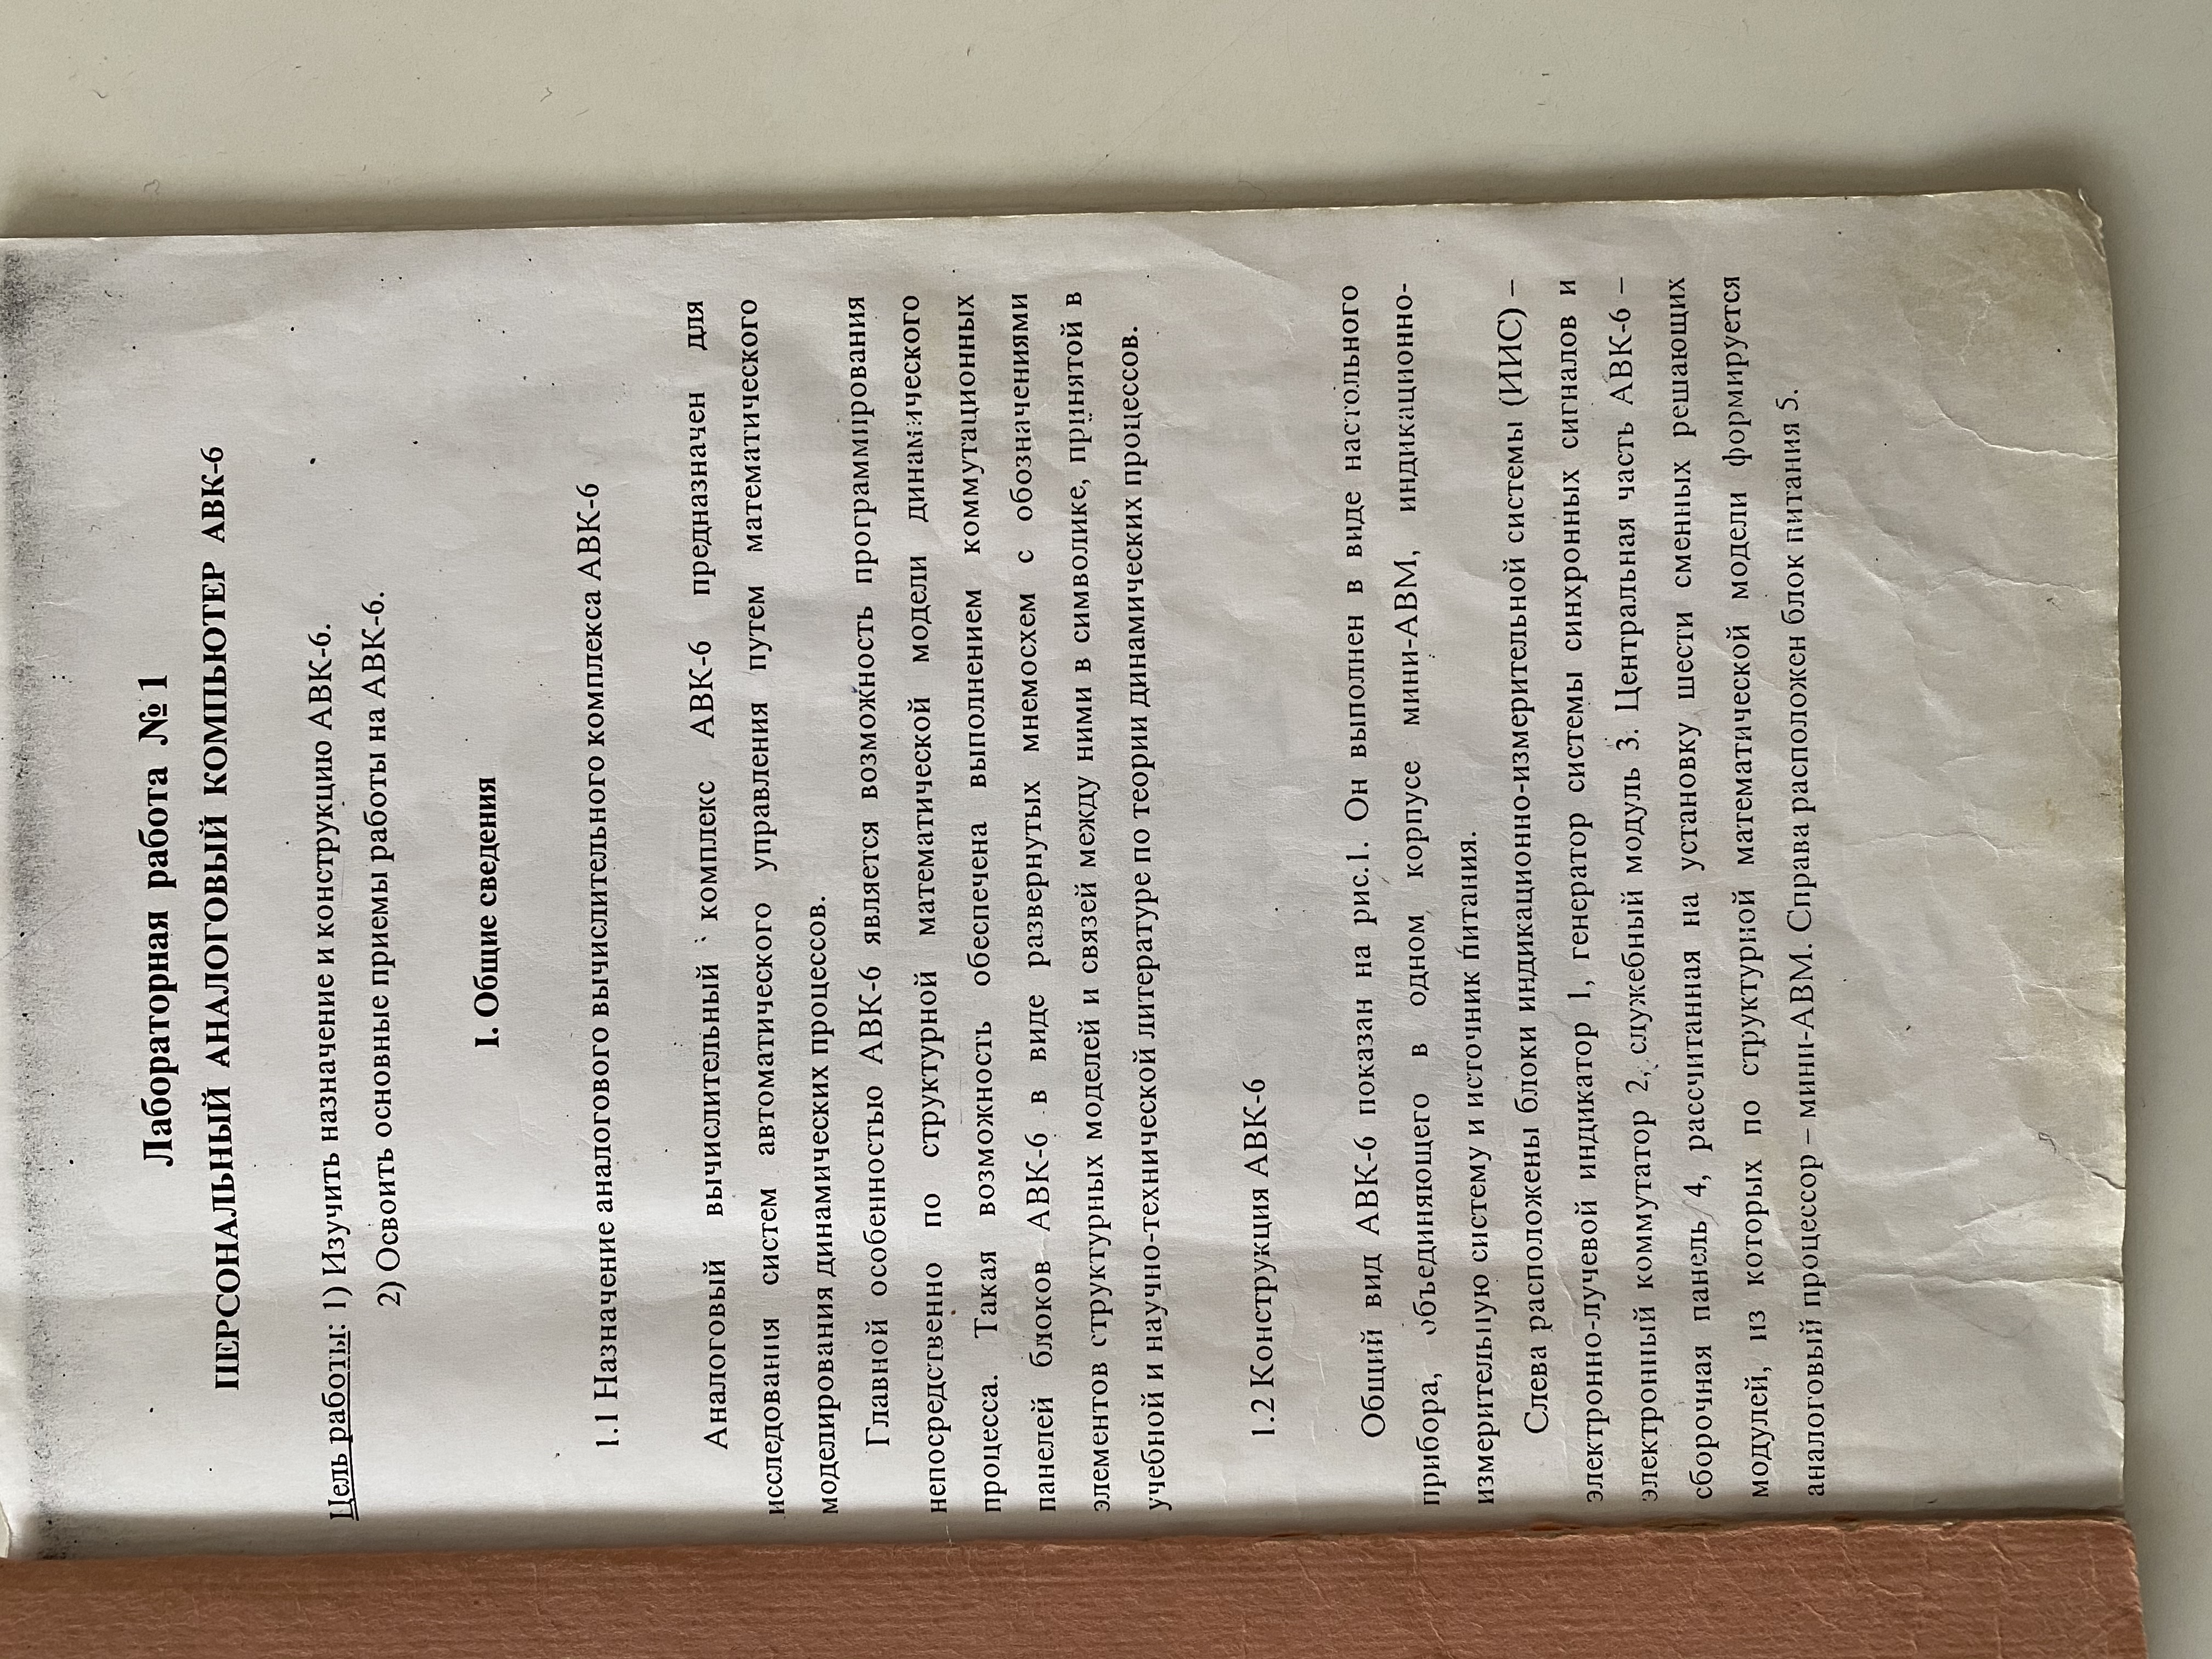
\includegraphics[width = \columnwidth]{./assets/p01.png}
        \caption{Результат виконання розробленої програми}
        \label{fig:app-res}
      \end{figure}

      Як~видно, програма коректно обчислює значення заданого виразу з~вхідними значеннями, заданими у~програмі.

  \section{Висновок}
		Виконуючи дану лабораторну роботу, ми~розробили програму для~заданої паралельної комп'ютерної системи із~локальною пам'яттю, ознайомились із~процесом розробки паралельних алгоритмів, а~також із~обміном повідомленнями за~допомогою програмного інтерфейсу~\textenglish{\allcaps{MPI}}.

  \newpage
  \appendix
  \section{Програма для~розв'язку поставленої задачі}

    \inputpython{../01-solution/solution.py}{Початковий код~програмного модуля для~розв'язання задачі}{lst:source-code}

\end{document}
